\documentclass[a4paper,12pt]{article}
\usepackage{mathrsfs}
\usepackage{geometry}
\usepackage{tcolorbox}
\geometry{a4paper,left=2.5cm,right=2cm,top=2cm,bottom=2cm}

\begin{document}
	\section{Purpose of this DAQ ?}
	I wrote this DAQ in the hope for it to become the (prototype of)
	standard DAQ used by IMP. As far as I learned, by the time this DAQ was
	written, no `standard' DAQ existed in IMP and nobody was working on
	this, even (probably) nobody was thinking about such a thing. This is,
	in my humble opinion, one major thing that we were behind others (e.g.
	GSI, NSCL/FRIB). However, to really develop a universal DAQ applicable
	to many experiments, we may need a whole group to do that. I cannot do
	that on my own. So in this version of DAQ, I kept many things as simple
	as possible and many things remained unoptimized. The bottom line was to
	make sure that it works and can be easily used by others. How easy could
	it be ? Well, in most cases, one should be able to set it up by just
	clicking mouse and fill in some parameters (like module base addresses)
	without any coding (except for the online analysis part). To that end,
	one has to use only the modules predefined in this DAQ, unsupported
	modules won't work properly (in fact, they won't work at all). What if
	one needs to use an unsupported module? There are three ways to work it
	around: i) find an alternative module; ii) contact me to include your
	module (gaobsh@impcas.ac.cn); iii) do it yourself, you should be able to
	include your module easily since special care was taken to accomplish
	that.

	Part of the DAQ designment is inspired by the NSCL DAQ.

	\section{Overview of the DAQ}
	\begin{figure}
		\begin{center}
			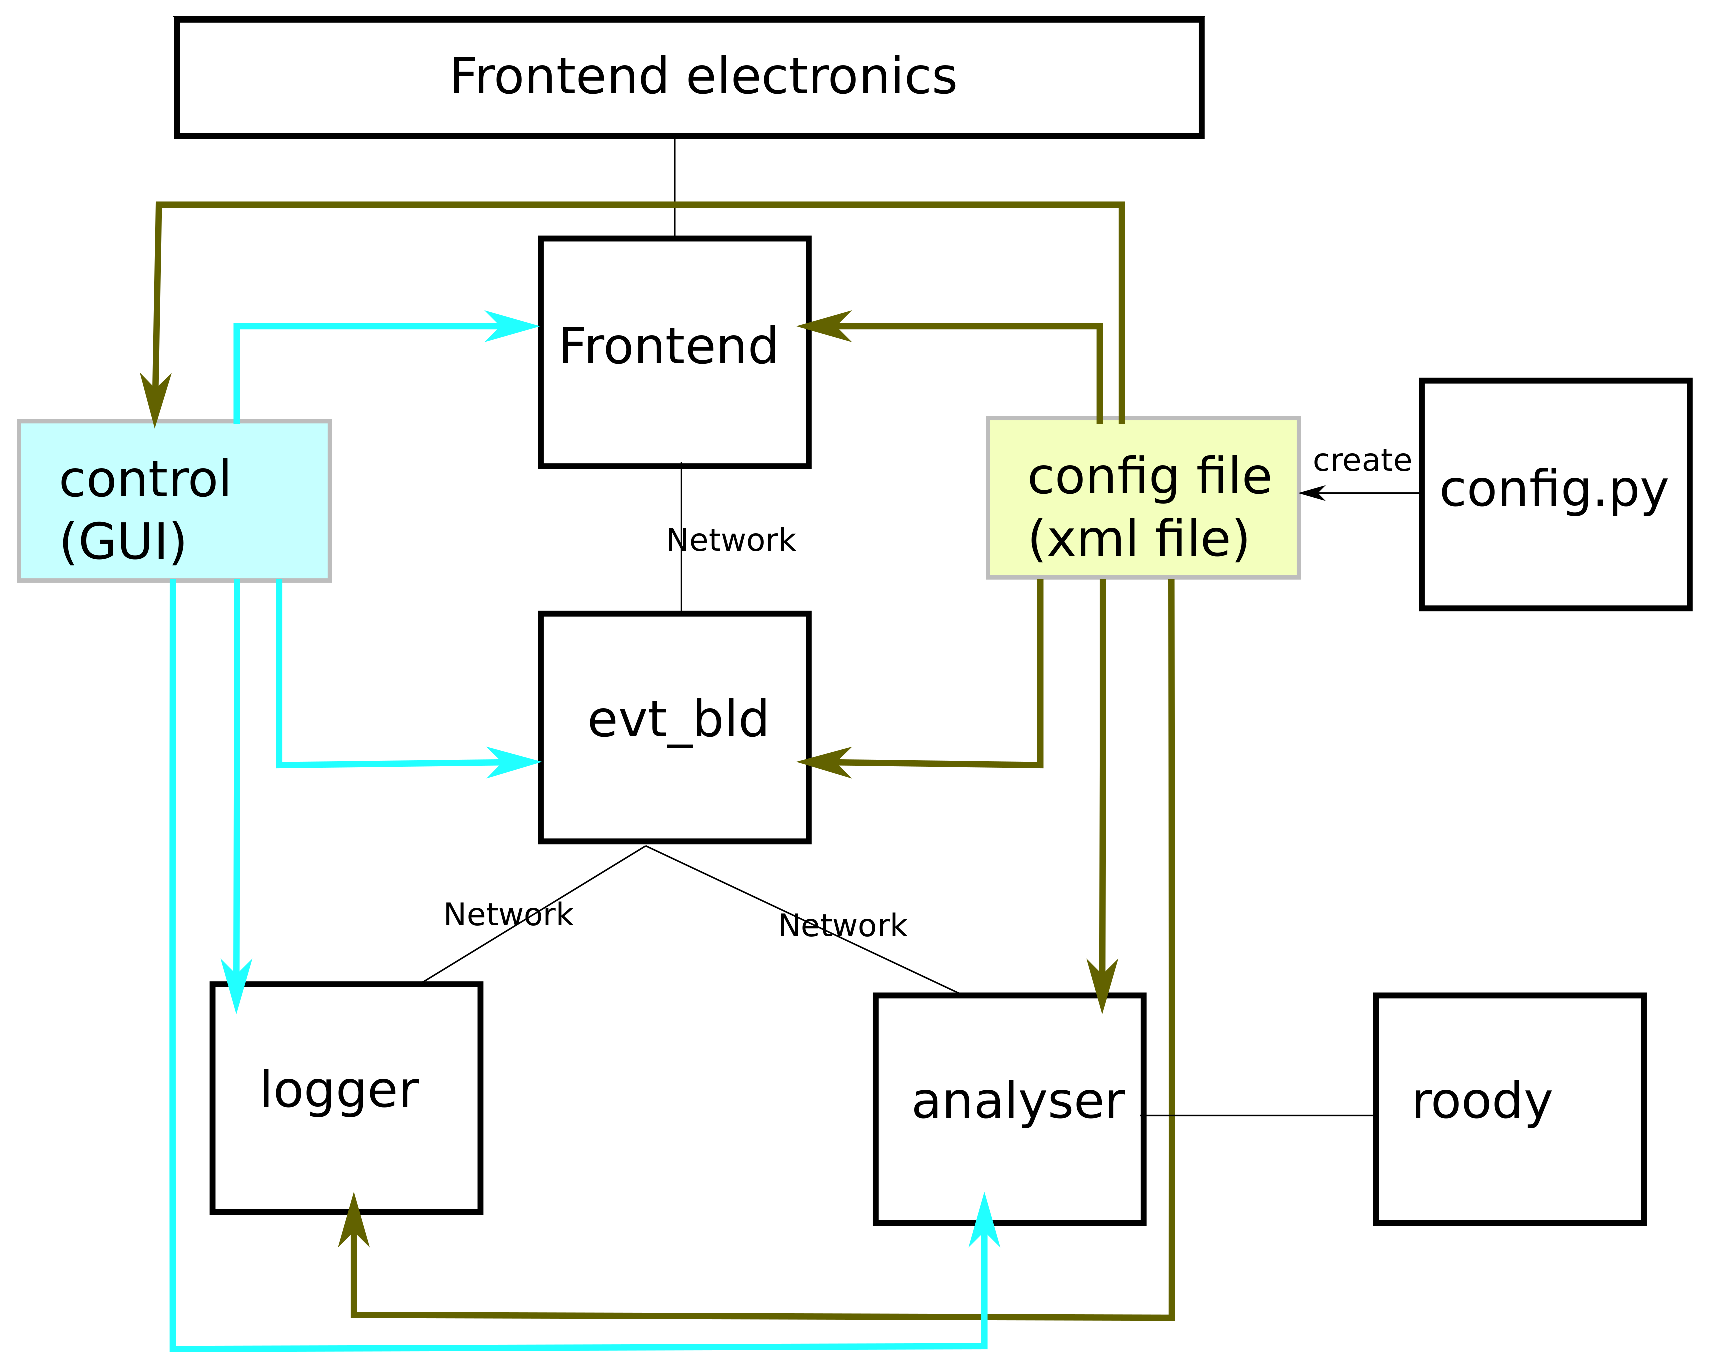
\includegraphics[width=.7\textwidth]{figs/daq_scheme.eps}
			\caption{\label{fig01}Components of the DAQ }
		\end{center}
	\end{figure}
	This DAQ consists of the following parts, see Fig. \ref{fig01}:
	\begin{itemize}
		\item config. This is a GUI program (python script) to help user
			create the configuration file used by the DAQ. The configuration
			file (xml file) contains all the information needed to setup the
			DAQ (used modules, base addresses, register settings of modules,
			etc.).
		\item frontend. This is the part that communicates with the
			electronics (e.g. VME modules).
		\item evt\_bld. This is the event builder. It receives data from the
			frontend and build a complete event based on timestamps of the
			fragments readout by frontend.
		\item logger. This program takes data from evt\_bld and records it
			in hard drives.
		\item analyser. This program also takes data from evt\_bld, it
			analysis the events and makes histograms instead of recording
			them.
		\item roody. This program displays the histograms made by the
			analyser. Strictly speaking, roody is not really part of the
			DAQ. It should be seen as a `hist displayer'.
		\item control. This is a GUI program which controls the running of
			the DAQ (e.g.  start, stop, quit...) and shows statistics (e.g.
			kb/s, loads of ring buffers...). It also receives messages from
			other components and save it into files (and/or show it on the
			screen). It can also sample data from ring buffers of other
			components and print it out (for debugging).
	\end{itemize}
	The communications between different programs is done via sockets. This
	makes it easier to combine two DAQs into one as shown in Fig.
	\ref{fig02}. Combining multipole DAQs involves the following
	modifications:
	\begin{itemize}
		\item The slave DAQ(s) don't have the event builder and the
			subsequent components, the data readout by its frontend are send
			to the event builder of the master DAQ.
		\item To enable the event builder and subsequent components of the
			master DAQ work properly, they need read the configuration file
			of the slave DAQ(s) too.
		\item Because the event builder build events based on time stamps,
			the clocks of the DAQs should be synchronized.
	\end{itemize}
	\begin{figure}
		\begin{center}
			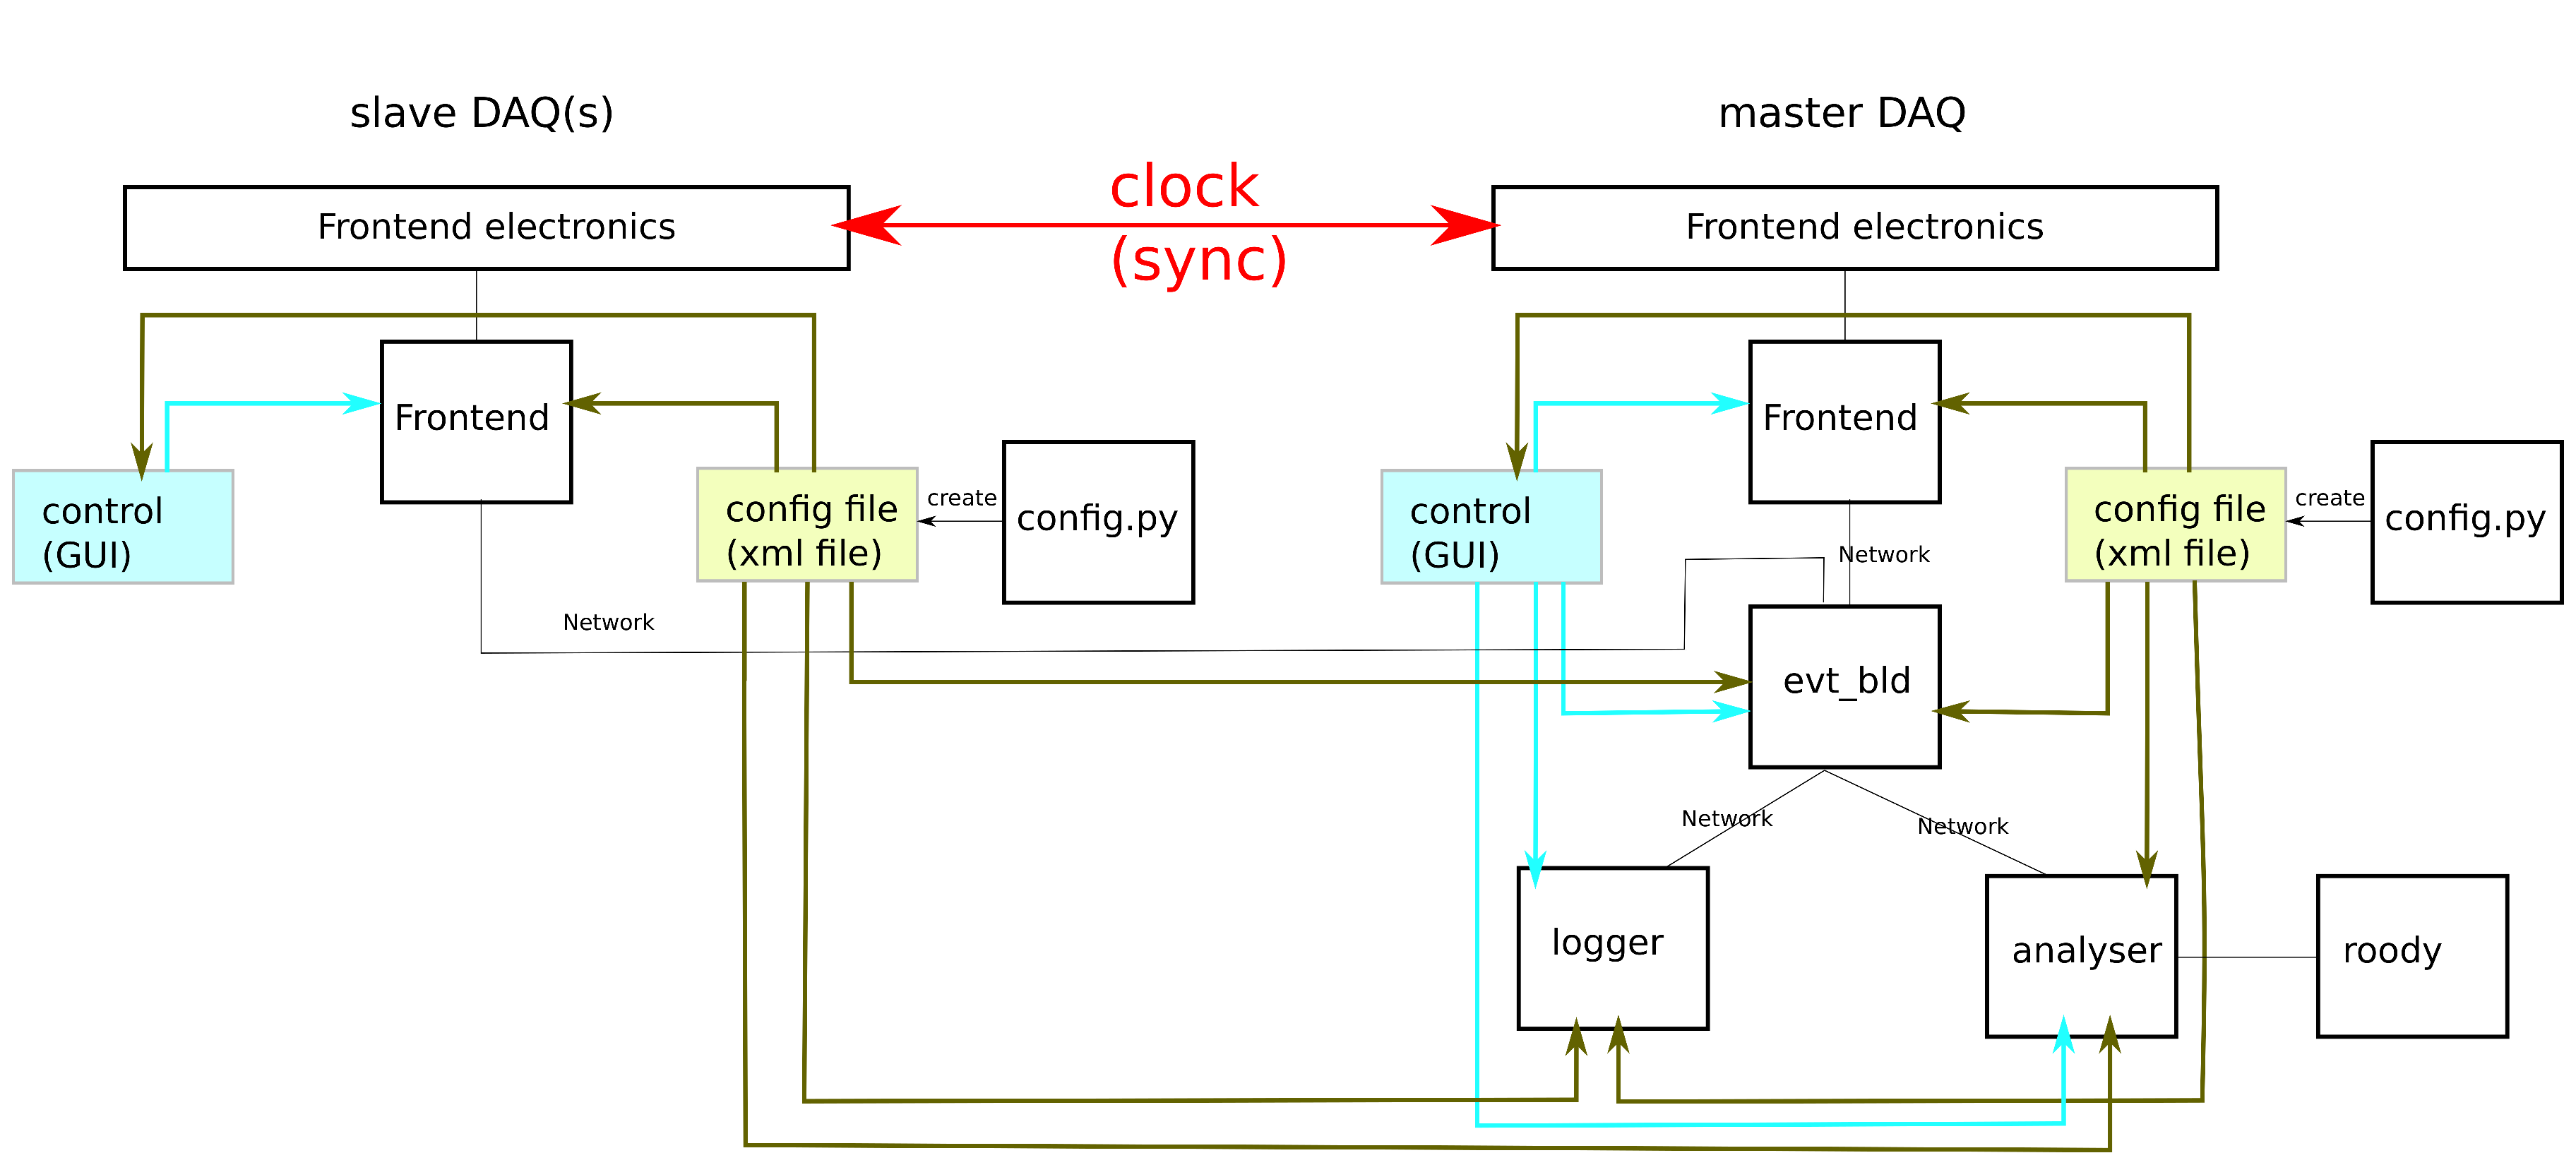
\includegraphics[width=.9\textwidth]{figs/daq_scheme2.eps}
			\caption{\label{fig02}Configuration of the DAQ with two DAQs}
		\end{center}
	\end{figure}
	The basic requirement is that all the supported modules (trigger type)
	should have time stamps for each event, so that the event builder can
	build events based on their time stamps. However, there should be some
	mechanism that allows user to use modules that don't have time stamps
	(may at the cost of significantly downgraded performance though).


	\section{Frontend}
	The first question about frontend is how to (possibly) write a frontend
	which can be applicable in various experiments using various modules ?
	The basic idea is to include all supported modules in the code, then
	select those used in real experiments by using $if$ statements. To be
	more specific, the frontend can be thought of as doing the following
	things: i) initialize modules, ii) wait for trigger, iii) readout data
	and goto last step again. So for example what we are going to do in step
	iii is to read out data from all the modules that are actually used in
	the experiment. How do we know which modules are used ? We can find it
	out from the configuration file.

	Since frontend will communicate with the electronics, connections of the
	hardware is needed to run the program. However, for testing purposes, it
	should provide a mechanism to run the program without really connecting
	the hardware electronics (just to see if the DAQ works at all).
	
	The main task of frontend is to read data from modules and send the data
	out to event builder with minimum pre-processing. The modules can be
	categorized into two types: `trigger type' and `scaler type'. The
	`trigger type' modules are read whenever there is a trigger, the `scaler
	type' modules are read regularly, independent of the trigger. Meanwhile
	the frontend has to communicate with the controller. So four threads
	should be used:
	\begin{itemize}
		\item Thread 1, (main thread). It waits for trigger and read data
			from modules. Then it packs and copies the data into a ring
			buffer.
		\item Thread 2. It reads data regularly from scaler type modules and
			packs and copies the data into the ring buffer as in thread 1.
		\item Thread 3. It reads data packets from the ring buffer and sends
			them out to the event builder (Tcp server).
		\item Thread 4. It communicates with the controller (Tcp client).
	\end{itemize}

	\section{event builder}
	\begin{figure}
		\begin{center}
			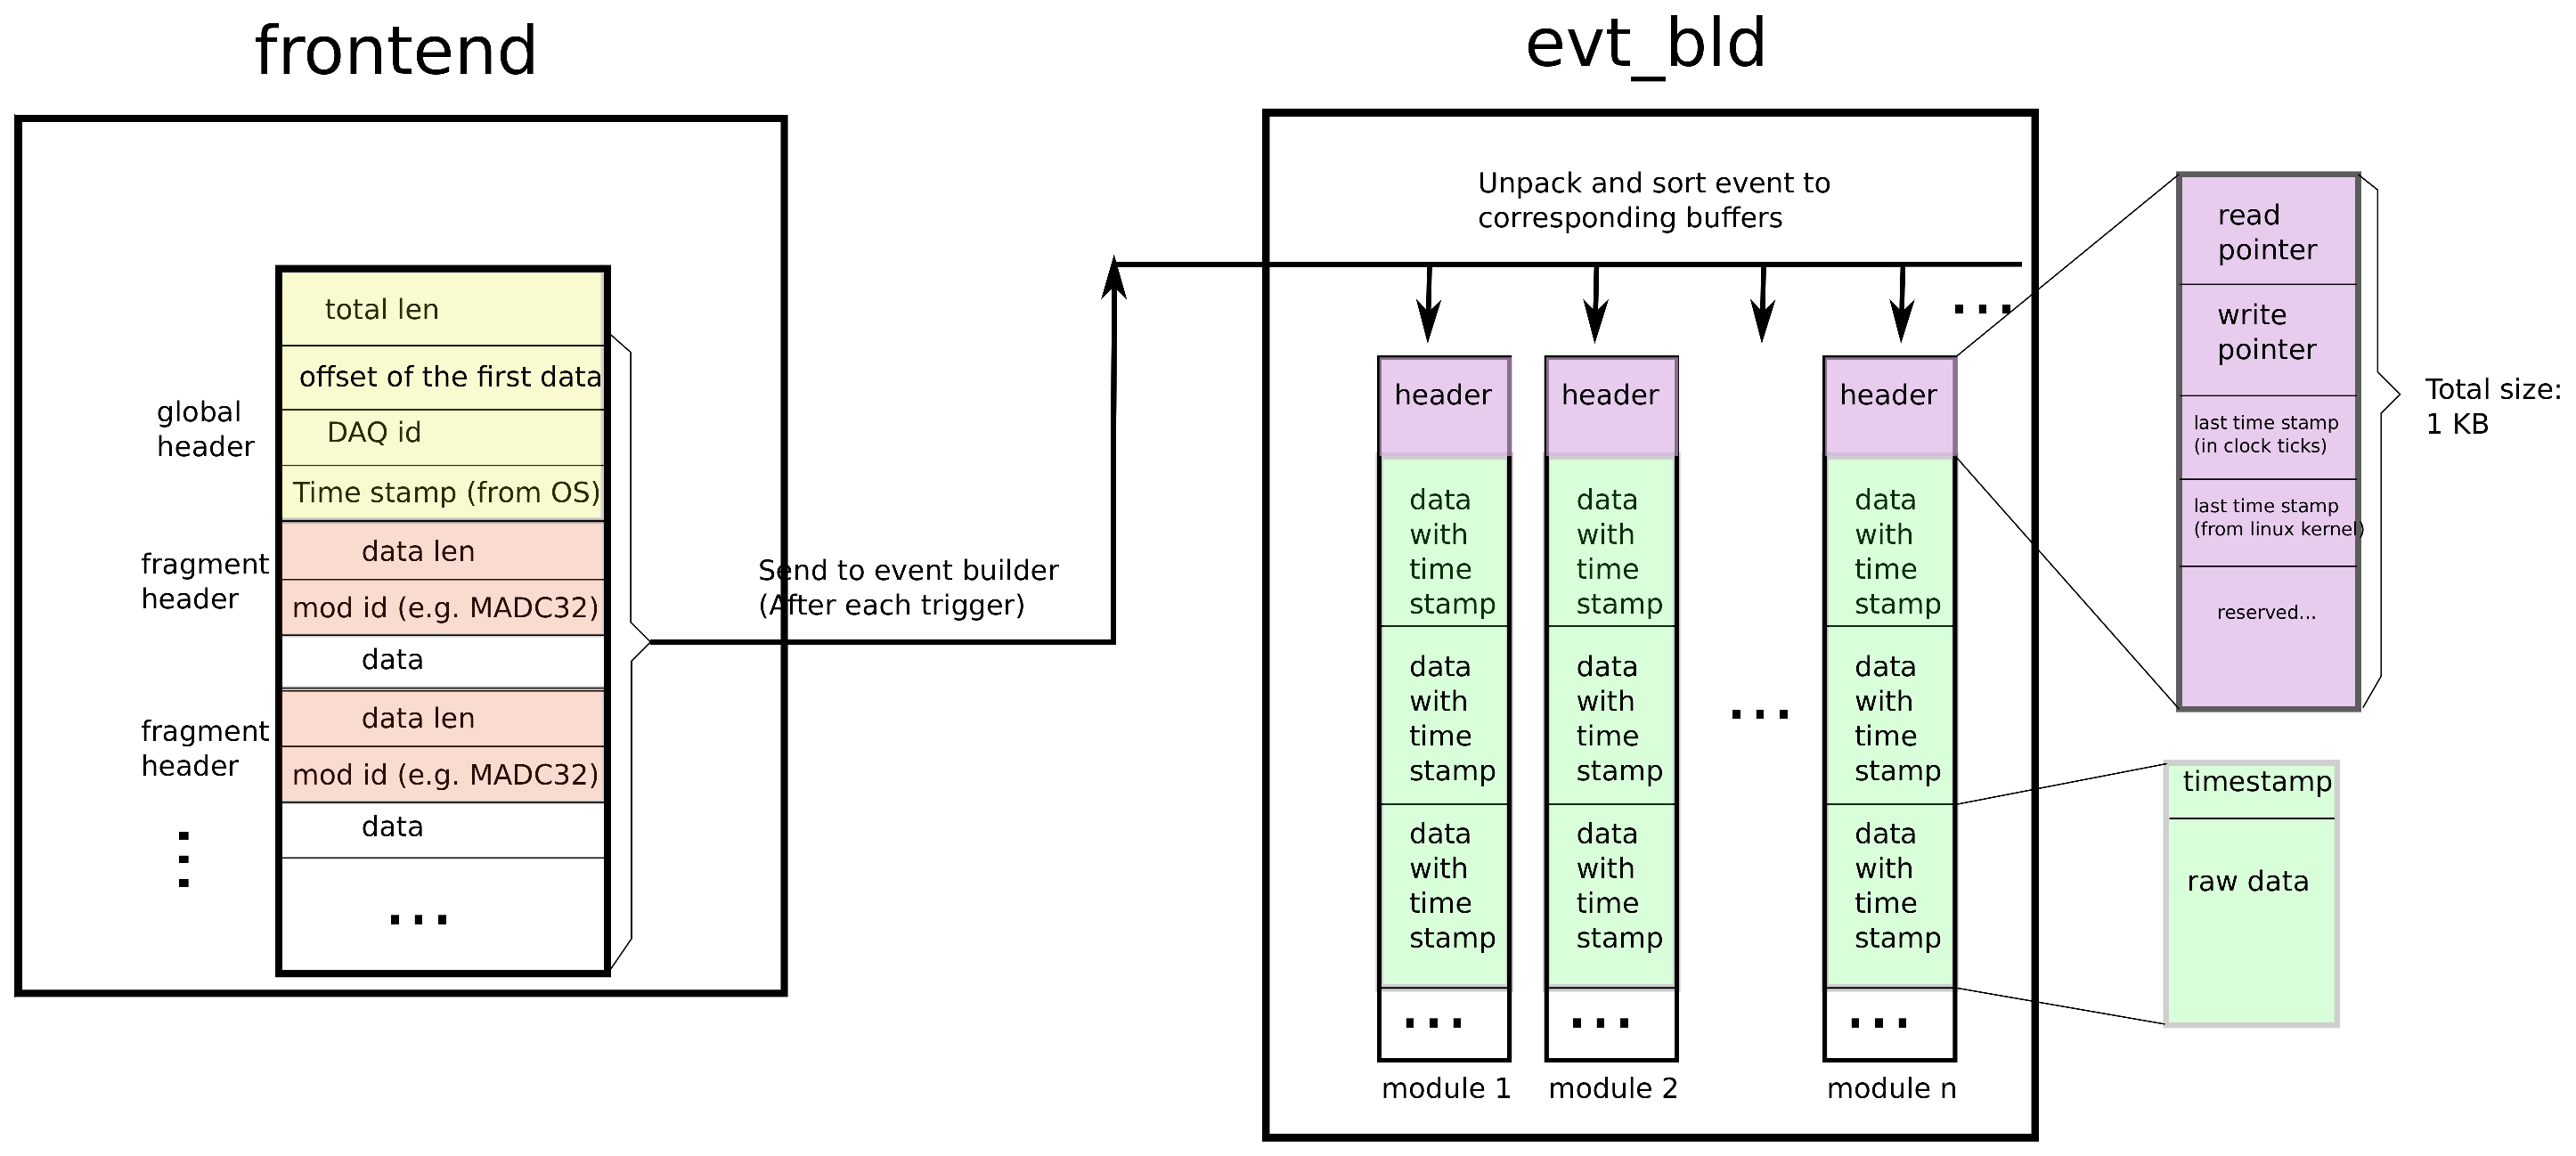
\includegraphics[width=.9\textwidth]{figs/data_format.eps}
			\caption{\label{fig03}Data flow in the event builder }
		\end{center}
	\end{figure}
	The main task of event builder is to build event from the data received
	from frontend based on their time stamps. Four threads should be used:
	\begin{itemize}
		\item Thread 1. It receives data from frontend (Tcp client). Then it
			sorts the data into different ring buffers. Here each single
			module (adc, tdc ...) has a dedicated ring buffer. In each ring
			buffer, the events are sorted by their time stamps.
		\item Thread 2 (main thread). It reads data from the ring buffers in
			thread 1 and build events out of the fragments contained in the
			ring buffers. It then copies the composed event into the `master
			ring buffer'.
		\item Thread 3. It read the composed events from the `master ring
			buffer' and sends them out to logger \& analyser (Tcp server).
		\item Thread 4. It communicates with the controller (Tcp client).
	\end{itemize}
	The processing of the data flow is demonstrated in Fig. \ref{fig03}.

	\section{Analyzer}
	This is the online analysis of the experimental data. It receives
	(composed) events from the event builder and do meaningful analysis and
	fill user defined histograms. However, the displaying of histograms are
	done by another program `roody' (see next section).
	Four threads should be used in analyser:
	\begin{itemize}
		\item Thread 1. It receives events from event builder and save them
			in a ring buffer.
		\item Thread 2 (main thread). It analysis the events stored in the
			ring buffer and fill the user defined histograms.
		\item Thread 3. It communicates with the histogram displayer (Tcp
			server). For example it sends data to and receives requests from
			the displayer (roody).
		\item Thread 4. It communicates with the controller (Tcp client).
	\end{itemize}
	Analyser is the only program that needs user coding, so the source files
	should be organized such that the user coding file is clearly separate
	from the other back end files. For this purpose, a file named
	user\_code.cpp should be used for the user code. In this file two
	functions exists for the user to modify: book\_hists() and
	do\_analysis(). The  book\_hists() defines histograms that the user
	wants to see from the online analysis. The do\_analysis() receives a
	pointer to an event and do whatever analysis the user wants, and then
	fill the histograms. Note: when filling the histograms, synchronization
	should be considered because thread 3 may also be reading the
	histograms.

	\section{roody}
	Roody is developed by the TRIUMF
	(https://www.triumf.info/wiki/DAQwiki/index.php/ROODY). It is better to
	get a stable working version (based on the same version of root as
	Analyser, preferably root version of 5.32) and not to change that. 

	\section{control}
	The program control (a python script) is the controller of the whole
	DAQ. Since it is just a controller of the DAQ, it should be designed
	such that the DAQ is OK if the control program exited (unexpectedly).
	For example, we can launch the DAQ without launching the controller at
	all (however we have no control over the DAQ though, e.g. to start a
	run).  We can also start a run using the control then exit the
	controller, then we can launch the controller again and everything
	should be as if we haven't exited the controller. The controller
	performs the following tasks:
	\begin{itemize}
		\item Controls the status of the DAQ (start, stop, quit).
		\item Receives messages from other components of the DAQ and save it
			to files. 
		\item Shows the statistics of the current run (e.g. kb/s, ring buffer
			loads, free disk space...)
		\item Shows the samples of the data in the ring buffers (for
			debugging).
	\end{itemize}
	To accomplish the above tasks, it should be like \ref{fig04}.
	\begin{figure}
		\begin{center}
			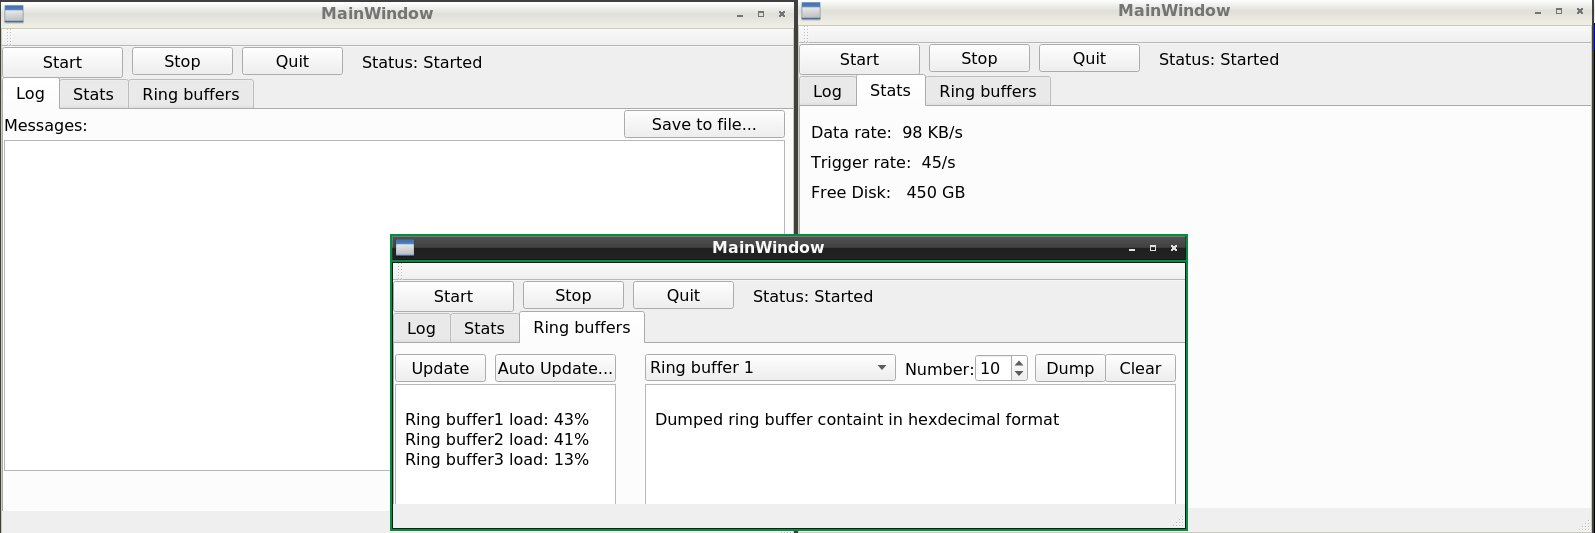
\includegraphics[width=.9\textwidth]{figs/control.eps}
			\caption{\label{fig04}The program `control'}
		\end{center}
	\end{figure}
	The widgets are:
	\begin{itemize}
		\item Start (button). When pressed, a dialog should be popped up
			asking for the run number and the title, then start a new run.
			When the DAQ status is already `Started', this button should be
			disabled to prevent double start.
		\item Stop (button). When pressed, a dialog should be popped up
			asking like `are you sure to stop ?', when confirmed, stop the
			current run.  When the DAQ is already `Stopped', this button
			should be disabled to prevent double stop.
		\item Quit (button). When pressed, a dialog should be pooped up
			asking like `are you sure to quit ?', when confirmed, quit the
			whole DAQ.  The button should be disabled if the DAQ is
			currently started, i.e. the user can quit the DAQ only if it is
			stopped.
		\item Status (label or text box). This shows the current status of
			the DAQ: either started or stopped. For simplicity, we don't
			provide `paused' status. To obtain the status, the control
			program should query the frontend (i.e. the control itself
			should not keep track of the status of the DAQ, the frontend
			should do that).
		\item The log page (page). It contains two widgets:
			\begin{itemize}
				\item Messages (read only text box). It shows the messages
					received from other components of the DAQ.
				\item Save to file... (button). When clicked, a dialog
					popped up asking for the file name to save the contents
					in the Messages, then save the messages.
			\end{itemize}
		\item Stats (page). It contains a read only text box showing the
			following information:
			\begin{itemize}
				\item Data rate.
				\item Trigger rate.
				\item Free disk space.
				\item Something else... (To be added on demand).
			\end{itemize}
		\item Ring buffers (page). It contains the following widgets:
			\begin{itemize}
				\item Update (button). When clicked, update the ring buffer
					loads shown in the text box below the button. Because
					this ring buffer information is mainly used for
					debugging purposes, it is not supposed to be updated
					very frequently. 
				\item Auto Update...(button). When clicked, a dialog pops up
					asking for the update frequency of the ring buffer
					loads, then update the loads automatically according to
					the frequency.
				\item Ring buffer loads (read only text box). It shows the
					load of each ring buffer (occupancy percentage of the
					buffer).
				\item Ring buffer name (ComboBox). It selects the ring
					buffer whose contents are to be dumped. 
				\item Number (SpinBox). It sets the number of items in the
					ring buffer to dump.
				\item Dump (button). When clicked, the contents of the
					specified ring buffer is dumped in the text box below
					the button (in hexadecimal format)
				\item Clear (button). When clicked, a dialog pops up asking
					for confirmation, then clears the contents of the text
					box below the button.
				\item Dumped contents (read only text box). It shows the
					dumped contents of a ring buffer in hexadecimal format.
			\end{itemize}
	\end{itemize}
	
	\section{config}
	This program create a configuration file (or modifies an existing one)
	used by all other components of the DAQ. All information needed to run
	the DAQ is contained in the configuration file which is a xml file.
	
	The $config$ program should look like Fig. \ref{fig05}. It includes
	several pages of which the $Frontend$ page is most important and
	provides the most crucial information. It includes the following
	widgets:
	\begin{itemize}
		\item Open... (button). When clicked, it pops up a window allowing
			the user to select the configuration file to be opened. In this
			case, we work on an existing file.
		\item Save (button). When clicked, the modifications are saved to
			the existing file. In case of new file, it pops up a window
			asking for the file name of the new (created) file and then save
			it.
		\item Supported Modules (list widget). In this list, all the
			supported modules are shown. 
		\item Add$==>$ (button). Add the selected module in the left list into
			the right list (Selected modules). All the settings of the added
			module is set to its default values.
		\item Selected Modules (list widget). In this list, all the selected
			modules are shown and these modules are to be used in the DAQ.
			The letters (T) and (S) indicates their type (T for trigger type
			and S for scaler type). When double click on one item, a window
			pops up for the user to modify the settings of the item
			(module). Right click the item allows the user to remove,
			duplicate (and maybe some other operations) the module. 
		\item New Crate (button). When clicked, a new crate is created
			allowing user to add modules to a new crate.
		\item Advanced... (button). When clicked, it pops up a window for
			more advanced settings of the frontend. These settings are
			usually not supposed to be modified by most users.
		\item Move up/ Move Down (button). It allows the user to change the
			slots of the selected item in the `Selected Modules' list.
	\end{itemize}
	\begin{figure}
		\begin{center}
			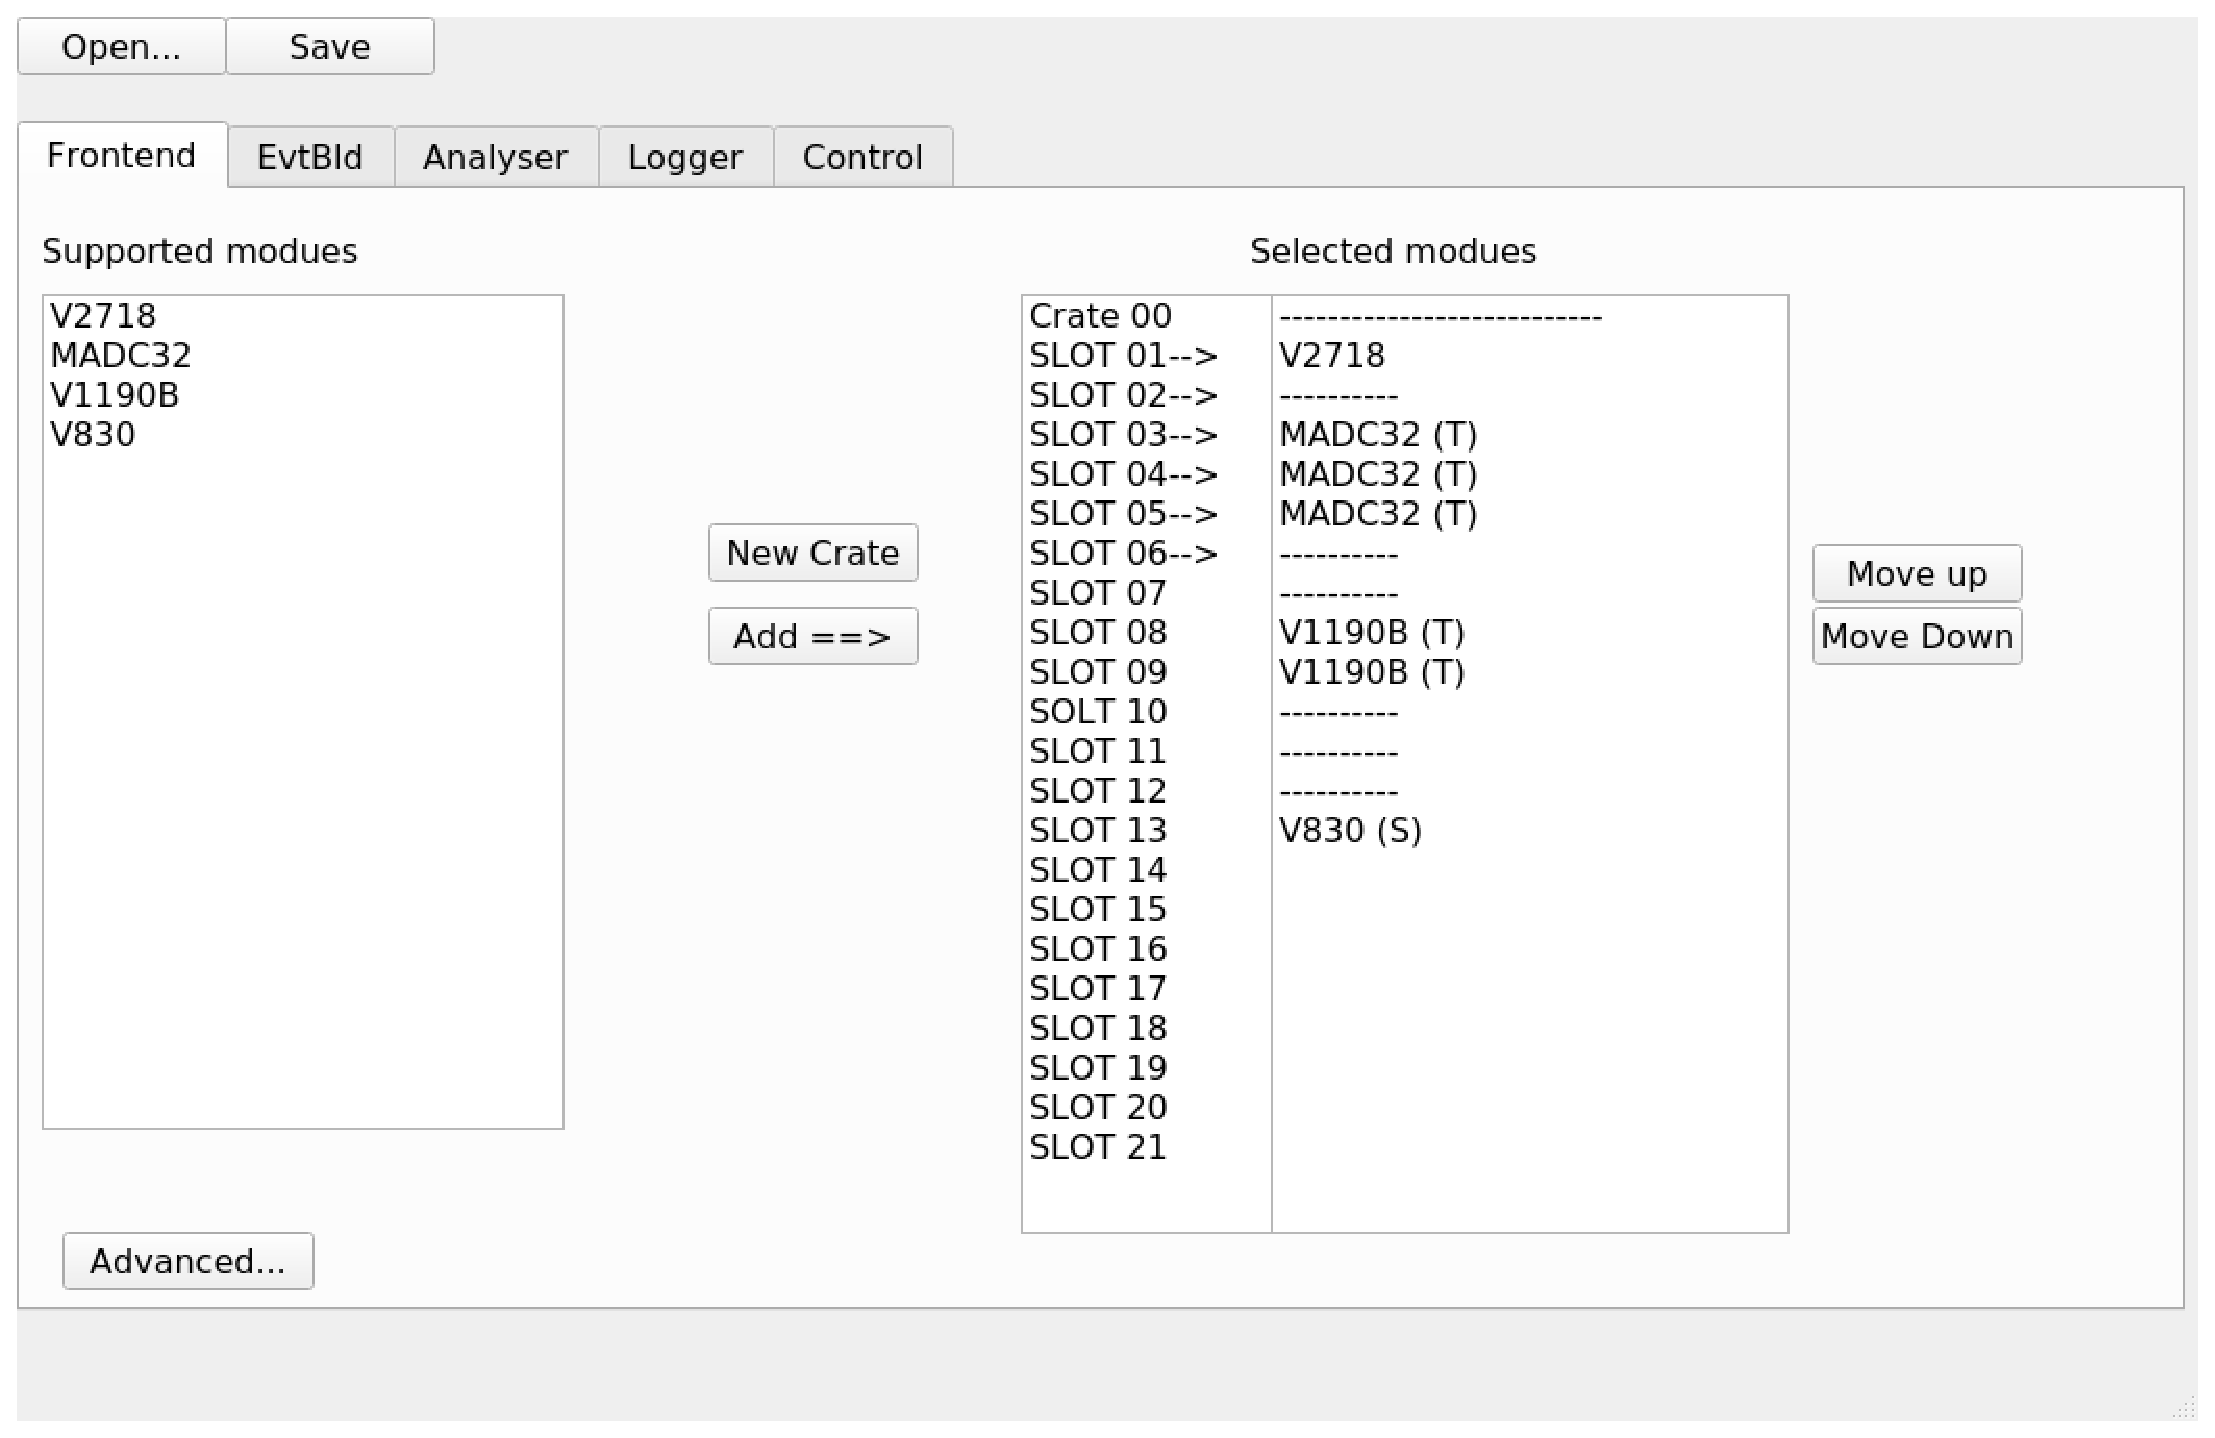
\includegraphics[width=.9\textwidth]{figs/config.eps}
			\caption{\label{fig05} The $config$ program. }
		\end{center}
	\end{figure}



\end{document}
